\documentclass[a4paper, 11pt]{article}
\usepackage[utf8]{inputenc}
\usepackage[czech]{babel}
\usepackage{amsmath}
\usepackage[dvipsnames,table]{xcolor}
\usepackage{tipa}
\usepackage{graphicx}
\graphicspath{{.}}
\usepackage{enumitem}
\usepackage[a4paper, left=20mm, top=30mm, text={170mm, 240mm}]{geometry}

\setlength{\parindent}{0em}
\setlength{\parskip}{1em}

\providecommand{\nonterm}[1]{\textless \textbf{#1}\textgreater}
\providecommand{\term}[1]{\textcolor{Green}{\textbf{#1}}}
\providecommand{\arrow}{ $\rightarrow$ }
\providecommand{\E}{ \textcolor{Orange}{\textbf{E}}}
\providecommand{\eps}{ \textcolor{Red}{\textbf{\textepsilon}}}

\definecolor{light-gray}{gray}{0.95}


\begin{document}
    \begin{titlepage}
        \begin{center}
        \textsc{{\LARGE Vysoké učení technické v~Brně\\[0.3em]
        Fakulta informačních technologií}}\\
        \vspace{\stretch{0.382}}
        {\Huge \textbf{Formální jazyky a překladače}\\2016/2017}\\[1em]
        {\LARGE \textbf{Dokumentace interpretu imperativního jazyka IFJ16}}\\[0.5em]
        {\Large \textbf{Tým 013, varianta b/3/I}\\[0.3em]Rozšíření: BOOLOP}
        \vspace{\stretch{0.618}}
        \end{center}
        {\large
        \begin{tabular}{l l l l}
            Šuba Adam & xsubaa00 & 25\% & vedoucí týmu\\
            Paliesek Jakub & xpalie00 & 25\% &\\
            Šuhaj Peter & xsuhaj02 & 25\% &\\
            Tóth Adrián & xtotha01 & 25\% &\\
        \end{tabular}}
        \\
        \begin{flushright}
        11.\,12.\,2016
        \end{flushright}
    \end{titlepage}

    \tableofcontents\newpage

    \section{Úvod}
    \par
    Dokumentace popisuje vývoj interpretu imperativního jazyka IFJ16. Jazyk IFJ16 je podmnožinou jazyka Java SE 8, což je staticky typovaný, objektově-orientovaný jazyk.
    Úlohou našeho interpretu je kontrola zdrojového kódu napsaného v jazyku IFJ16 a jeho následná interpretace.\par
    Zvolená varianta zadání Tým 013 má parametry b/3/I:
    \begin{itemize}[itemsep=1mm]
        \item(b) vyhledávání podřetězce s použitím Boyer-Mooreova algoritmu
        \item(3) řazení s použitím algoritmu Shell sort
        \item(I) implementace tabulky symbolů použitím binárního vyhledávacího stromu
    \end{itemize}
    Dokumentace je rozdělená na kapitoly, které blíže popisují jednotlivé části interpretu a způsob jejich řešení. Taktéž obsahuje i popis použitých algoritmů, rozdělení úloh a způsob práce v týmu. V závěru dokumentace se nachází shrnutí naší práce.\\
    V příloze se nachází:
    \begin{itemize}[itemsep=1mm]
        \item diagram konečného automatu lexikální analázy
        \item LL-gramatika pro syntaktickou analázu shora dolů
        \item precedenční tabulka pro syntatickou analýzu zdola nahoru
    \end{itemize}
    
    \section{Návrh}
    Plánování procesu vývoje interpretu nám bylo značně zjednodušeno závazně zadanými metodami implementace synktatické analýzy. V případě metody zhora dolů jsme se rozhodli pro rekurzivní sestup.\par
    Samotný vývoj jsme naplánovali na 6 fází, s cílem mít při pokusném odevzdání plně funkční produkt.
    \begin{enumerate}[itemsep=0mm]
        \item Vývoj lexikálního analyzátoru
        \item Vývoj syntaktického analyzátoru
        \item Příprava tabulky symbolů
        \item Vývoj sémantické analýzy a její integrace do syntaktického analyzátoru
        \item Vývoj interpretu
        \item Dokončení a vyladění celého produktu, tvorba dokumentace
    \end{enumerate}
    Vývoj lexikálního analyzátoru zahrnuje přípravu konečného automatu rozpoznávajícího lexémy jazyka IFJ16 a jeho implementaci. První části vývoje syntaktického analyzátoru je implementace rekurzivního sestupu. To vyžaduje tvorbu LL-gramatiky a LL-tabulky. Druhou částí je implementace precedenční analýzy, která vyžaduje tvorbu precedenční tabulky. V mezičase je možné navrhnout a implementovat tabulku symbolů a připravit sémantickou analýzu pro integraci do synaktického analyzátoru. Jakmile je hotová kontrola správnosti vstupního programu a jsou generovány instrukce, je možné přistoupit k implementaci interpretu. V průběhu vývoje jednotlivých modulů jsou připravovány testy jak samotných modulů, tak jejich spolupráce s ostatními moduly. Závěrečná fáze zahrnuje odstranění co nejvíce chyb a tvorba dokumentace.
    \section{Interpret}
    Implementaci interpretu lze rozdělit do 5 logických celků. Hlavní komponentou je syntaktický analyzátor, neboli \uv{parser}, který řídí činnost lexikálního analyzátoru, \uv{scanneru}, a také provádí sémantické akce sémantického analyzátoru. Sémantická analýza také vkládá informace o funkcicích a proměnných do tabulky symbolů. Poslední komponentou je samotný interpret, který provádí interpretaci instrukcí, vygenerovaných během kontroly vstupního programu.\par
    Kontrola správnosti programu je prováděna ve dvou průchodech, v prvním se některé části zdrojového kódu úplně ignorují (zéjména výrazy, které jsou závislé na sémantických akcích, více dále). Účelem prvního průchodu je naplnění tabulky symbolů.
    \subsection{Lexikální analyzátor}
    Jediným úkolem lexikálního analyzátoru je na žádost syntaktického analyzátoru přečíst další symbol ze zdrojového souboru, klasifikovat jej a předat ve formě tokenu zpět syntaktickému analyzátoru.\par
    Implementace je založena na konečném automatu. Bílé znaky a komentáře jsou ze zdrojového kódu odignorovány. Pokud řetězec dojde do koncového stavu reprezentující nějaký lexém a následující znak nepatří mezi znaky, které může daný lexém obsahovat a zárověň znak patří mezi znaky které mohou bezprostředně za daným lexémem následovat, je typ vraceného tokenu nastaven na typ odpovídající tomuto lexému. Některým tokenům je ještě přidělen atribut, obsahující užitečná data získaná z lexému. Pokud je v některém stavu přečten znak, který není v daném stavu podporován, popřípadě pokud je v koncovém stavu přečten znak, který nemůže následovat bezprostředně za daným lexémem, dojde k chybě. Poslední načtený znak, který rozhodl o ukončení konečného automatu, je vrácen zpět do vstupního souboru.\par
    {\small Poznámka:\\
    Při druhém průchodu syntaktické analýzy již není lexikální analyzátor činný. Při každém získání tokenu během prvního průchodu je daný token uložen do datového typu fronta a v druhém průchodu jsou tokeny brány z této fronty.}
    \subsection{Syntaktický analyzátor}
    Mozkem celé kontroly správnosti zdrojového kódu je synktatický analyzátor. Samotnou syntaktickou analýzu můžeme rozdělit do dvou částí: kontrola rekurzivním sestupem a kontrola správnosti výrazů precedenční analýzou.\par
    Rekurzivní sestup je metoda syntaktické analýzy shora dolů, která implementuje pravidla LL-gramatiky (viz příloha) na základě LL tabulky. Podle aktuálního stavu analyzátoru a vstupního tokenu je rozhodnuto, které pravidlo se zvolí. Metoda využívá rekurzivního volání funkce implementující dané pravidlo.\par
    Pro kontrolu správnosti výrazů se využívá precedenční analýza, která je metodou syntaktické analýzy zdola nahoru. Neboť bylo nutné nějakým způsobem napojit precedenční analýzu na rekurzivní sestup, přištoupili jsme k zavedení speciálního pseudoterminálu E do naší LL-gramatiky. V místě kontroly, kde by se měl nacházet tento terminál, se analyzátor přepne do režimu, kdy pouze žádá další a další tokeny a ukládá je do datového typu fronta. Tento režim je ukončen v moment, kdy narazí na token, který není ve výrazech podporován. Takto vytvořená fronta je poté předána precedenční analýze ke kontrole. Speciální případem, kdy je nutné lehce pozměnit chování tohoto procesu, jsou výrazy podmínek ve větvení a v cyklu. Zde je nutné počítat levé a pravé závorky tak, aby byl analyzátor schopen poznat, kdy nastal konec podmínky a fronta je naplněná. Samotná precedenční analýza je implementována podle algoritmu vyučovaném v předmětu IFJ. Abychom nemuseli do zásobníku uchovávajícího tokeny vkládat zarážku, vytvořili jsme ještě jeden pomocný zásobník, který v sobě ukládá ukazatele na místo, kde by se taková zarážka nacházela. Při redukci (pod)výrazu se poslední (tedy hledaná) zarážka nachází na vrcholu pomocného zásobníku.\par
    Neboť neimplementujeme rozšíření FUNEXP je pro nás funkce ifj16.print() speciální syntaktickou konstrukcí, neboť jí lze jako parametr dát jednoduchou konkatenaci, jejíchž výsledkem je vždy datový typ string. Z tohoto důvodu jsme se rozhodli nezahrnovat tohle chování do LL-gramatiky, ale vyřešit to jako speciální případ až při samotné implementaci analyzátoru. V druhém průchodu zdrojového souboru již díky sémantickým akcím analyzátor ví, že volaná funkce je ifj16.print() a na základě této informace se přepne do speciálního režimu, podobného přípavě na precedenční analýzu. Rozdíl je v tom, že povolené tokeny jsou pouze proměnné, literály a operátor konkatenace \uv{+}. Při ukončení tohoto režimu je zkontrolováno, zda-li alespoň jeden token byl typu string. Poté je konkatenace vyhodnocena precedenční analýzou. V naší implementaci je tedy tato jednoduchá konkatenace vyhodnocována zleva doprava podle stejných pravidel jako jiné výrazy. Výsledkem \texttt{3 + 5 + "$\backslash$n"} je tedy \texttt{"8$\backslash$n"} a nikoliv \texttt{"35$\backslash$n"}.\par
    \subsection{Sémantická analýza}
    Sémantická analýza je soubor funkcí a kontrol volaných během syntaktické analýzy v obou průchodech. V 1. průchodu do tabulky symbolů vkládá informace o třídách, statických funkcích, statických pro\-měnných, argumentech funkcí a kontroluje, zda nedošlo k redefinici. Těla funkcí nejsou v 1. průchodu sémanticky zpracována. V druhé fázi jsou pak generovány instrukce inicializačních výrazů statických proměnných a do tabulky symbolů jsou vkládány lokální proměnné. Rovněž jsou v této fázi zpracována těla funkcí, což zahrnuje kontrolu typů, kontrolu, zda byl identifikátor při jeho použití (u volání funkce, přiřazení) již definován a následné generování instrukcí, pokud nenastaly chyby zmíněné dříve.\par
    V případě sémantické správnosti kódu je během precedenční analýzy vždy při redukci části výrazu na neterminál generovaná aritmetická instrukce, případně i dodateční konverzní instrukce, pokud je daná implicitní konverze podporovaná. Výstupem sémantické akce generující aritmetickou instrukci je pomocná proměnná, která je během precedenční analýzy přiřazena jako atribut cílovému neterminálu a může být dále použita při jiné redukci.\par
    \subsection{Tabulka symbolů}\label{ts}    
    Tabulka symbolů (dále jen TS) je podle zadání implementovaná pomocí binárního vyhledávacího stromu. Vzhledem k tomu, že v jazyce IFJ16 existují různé rozsahy platnosti identifikátorů a třídy umožňují vytvářet oddělené jmenné prostory, navrhli jsme TS jako tříúrovňovou kaskádu vyhledávacích struktur. První úroveň je jediná tabulka tříd. Každá třída má potom vlastní tabulku členů (společnou pro statické proměnné a funkce). Funkce mají dále vlastní tabulky lokálních proměnných. \par
    Hodnoty statických proměnných jsou uložené přímo v odpovídajících položkách TS. Hodnoty lokálních proměnných nejsou, kvůli možnému rekurzivnímu volání funkcí, uložené přímo v TS, ale jejich hodnoty si ukládá interpret na svém zásobníku během vykonávání instrukcí.\par
    Různé typy proměnných (statická, lokální, pomocná) a literály jsou v naší implementaci reprezentovány různými strukturami, ale při sémantických akcích často není potřeba mezi nimi rozlišovat. Kvůli tomuto sme zavedli jednu extra strukturu, která je umístěna jako první člen ostatních struktur. Obsahuje informaci o tom, na kterou strukturu lze ukazatel na tuto univerzální strukturu dále přetypovat v případě potřeby. Je zde využita vlastnost jazyka C, že ukazatel na strukturu ukazuje na svého prvního člena a naopak.\footnote{http://www.open-std.org/jtc1/sc22/wg14/www/docs/n1124.pdf, s. 103} Krom toho ještě obsahuje informaci o datovém typu, který může sémantická analýza skontrolovat bez nutnosti přetypování.\par
    \subsection{Interpret}
    Interpret obsahuje jednu velkou funkci, jejímž vstupem je instrukční páska. Funkce se pomocí cyklu posouvá po instrukční pásce až do dosažení konce, tj. na instrukční pásce je \texttt{NULL}.\par
    Podle operačního kódu instrukce se zvolí příslušná větev interpretu a pomocná dekódovací funkce získá z instrukce operandy (jejich hodnotu, informaci o tom, jestli jsou inicializované apod.). Pro rámce funkcí má interpret svůj vlastní zásobník. Při volání funkce se vytvoří nový rámec, vyplní se potřebnými hodnotami (argumenty funkce, místo pro návratovou hodnotu, ukazatel na instrukci pro návrat) a vloží se na zásobník. Při návratu z funkce je návratová hodnota uložena na místa v rámci pro ni vymezeného a interpretace pokračuje od poznačené instrukce.
    \section{Algoritmy}
    Všechny popsané algoritmy jsou implementovány v souboru \texttt{ial.c}
    \subsection{Vyhledávání podřetězce použitím Boyer-Mooreova algoritmu (b)}
	Boyer-Moorův algoritmus je nejefektivnější algoritmus na vyhledávání podřetězce v řetězci. Vychází z klasického porovnávání hledaného vzorku patřičně přiloženému k prohledávanému řětěci, ale s tím rozdílem, že změna zarovnání vzorku s řetězcem se neděje po jednom, ale po více znacích. Porovnávání znaků přiloženého vzorku se děje od konce k počátku.\par
	K určení, o kolik znaků lze vzorek posunout (kolik zarovnání lze přeskočit), se používají dvě heuristiky. První z nich je heuristika \uv{bad character}, která se při neshodě snaží vzorek zarovnat tak, aby ke shodě došlo. Pokud to není možné (vzorek již daný znak neobsahuje), vzorek se zarovná až za daný znak v řetězci. Druhou heuristikou je \uv{good suffix}, která se v případě neshody po několika shodných znacích snaží vzorek zarovnat tak, aby nedošlo k porušení již nalezené shody. V naší implementaci jsme se rozhodli využít pouze první heuristiku.
    \subsection{Řazení použítím algoritmu Shell sort (3)}
    Shell sort je řadící algoritmus, který pracuje na principu bublinového vkládání. Neřadí prvky nacházející se výhradně vedle sebe, ale i posloupnosti oddělené určitým počtem prvků (krokem). V naší implementaci je na počátku tento krok stanoven na polovinu počtu prvků. Při každé další iteraci je hodnota kroku snížena na polovinu. V různých implementacích existují jiné způsoby určení těchto kroků, od čeho se odvijí jejich časová složitost. Algoritmus skončí jakmile krok dosáhne hodnoty 0. Shell sort pracuje \uv{in situ} a je nestabilní, což nám nevadí. Ve srovnání s jinými algoritmy je pomalejší než Quicksort a rychlejší než Heapsort. Složitost naší implementace je $O$(n$^2$).
    \subsection{Implementace tabulky symbolů použitím binárního vyhledávacího stromu (I)}
    Binární vyhledávací strom je binární strom, platí tedy, že je složen z kořene a levého a pravého podstromu. Všechny uzly nalevo od kořene mají klíče menší než kořen a všechny uzly napravo mají klíče větší než kořen. Vyhledávacím klíčem je v naší implementaci identifikátor symbolu. Funkce pro práci s binárními vyhledávacími stromy (v našem případě vyhledání uzlu, vložení uzlu a zrušení celého stromu průchodem PostOrder) byly implementovány rekurzivně. Implementace samotné tabulky symbolů byla popsána detailně v kapitole \ref{ts}.
    \section{Práce v týmu}
    \subsection{Rozdělení týmu}
    \begin{itemize}
        \item Adam Šuba – lexikální analyzátor, syntaktická analyza shora dolů a zdola nahoru, dokumentace, vedoucí
        \item Jakub Paliesek – sémantický analyzátor, tabulka symbolů, algoritmy, generátor 3-adresného kódu, dokumentace
        \item Peter Šuhaj – interpret, algoritmy, dokumentace
        \item Adrián Tóth – testy, algoritmy, dokumentace
    \end{itemize}
    \subsection{Způsob práce}
    Pro práci byl zvolen systém správy verzí Git, hostovaný na serveru GitHub. Kromě osobní komunikace byla hlavním komunukačním kanálem skupinová konverzace na sociální síti Facebook.
    \section{Závěr}
    Tým pracoval spolehlivě a časový plán se nám dařilo plnit. Jediné období, kdy nebylo možné na projektu aktivně pracovat bylo během půsemestrálního období, s čímž jsme ovšem během plánování počítali a problémy to tedy nezpůsobilo. Při prvním pokusném odevzdání jsme měli až na několik drobných chyb funkční interpret.
    \section{Literatura}
    \begin{enumerate}
    \item HONZÍK, Jan M., Algoritmy: Studijní opora. Verze: 16-B, Brno: Vysoké učení Technické, 2014
    \item https://cs.wikipedia.org/wiki/Shell\_sort
    \item ISO/IEC. ISO International Standard ISO/IEC 9899:TC2 – Programming Language C. Dostupné na http://www.open-std.org/jtc1/sc22/wg14/www/docs/n1124.pdf


    \end{enumerate}
    \newpage
    \section{Příloha}
    \subsection{LL-gramatika}
    \begin{enumerate}[itemsep=0mm]
        \item\nonterm{c-list}\arrow\term{class id \{ }\nonterm{memb-list}\term{ \}}       \nonterm{c-list}
        \item\nonterm{c-list}\arrow\term{\$}
        \item\nonterm{memb-list}\arrow\nonterm{c-memb} \nonterm{memb-list}
        \item\nonterm{memb-list}\arrow \eps
        \item\nonterm{c-memb}\arrow\term{static} \nonterm{c-memb1}
        \item\nonterm{c-memb1}\arrow\nonterm{type} \term{id} \nonterm{c-memb2}
        \item\nonterm{c-memb1}\arrow\term{void id} \nonterm{c-membfunc}
        \item\nonterm{c-memb2}\arrow\term{= }\E\term{ ;}
        \item\nonterm{c-memb2}\arrow\term{;}
        \item\nonterm{c-memb2}\arrow\nonterm{c-membfunc}
        \item\nonterm{c-membfunc}\arrow\term{(} \nonterm{fn-def-plist} \term{) \{} \nonterm{fn-body} \term{\}}
        \item\nonterm{type}\arrow\term{int}
        \item\nonterm{type}\arrow\term{double}
        \item\nonterm{type}\arrow\term{String}
        \item\nonterm{type}\arrow\term{boolean}
        \item\nonterm{fn-def-plist}\arrow\nonterm{par-def} \nonterm{fn-def-plist1}
        \item\nonterm{fn-def-plist}\arrow\eps
        \item\nonterm{fn-def-plist1}\arrow\nonterm{par-def} \nonterm{fn-def-plist1}
        \item\nonterm{fn-def-plist1}\arrow\eps
        \item\nonterm{par-def}\arrow\nonterm{type} \term{id}
        \item\nonterm{fn-body}\arrow\nonterm{stat} \nonterm{fn-body}
        \item\nonterm{fn-body}\arrow\nonterm{type} \term{id} \nonterm{opt-assign} \term{;} \nonterm{fn-body}
        \item\nonterm{fn-body}\arrow\eps
        \item\nonterm{stat-com}\arrow\term{\{} \nonterm{stat-list} \term{\}}
        \item\nonterm{stat-list}\arrow\nonterm{stat} \nonterm{stat-list}
        \item\nonterm{stat-list}\arrow\eps
        \item\nonterm{stat}\arrow\nonterm{id} \nonterm{as-ca} \term{;}
        \item\nonterm{stat}\arrow\nonterm{stat-com}
        \item\nonterm{stat}\arrow\term{if (}\E\term{ )} \nonterm{stat-com} \term{else} \nonterm{stat-com}
        \item\nonterm{stat}\arrow\term{while (}\E\term{ )} \nonterm{stat-com}
        \item\nonterm{stat}\arrow\term{return} \nonterm{ret-val} \term{;}
        \item\nonterm{id}\arrow\term{id}
        \item\nonterm{id}\arrow\term{fqid}
        \item\nonterm{as-ca}\arrow\term{( }\nonterm{fn-plist} \term{)}
        \item\nonterm{as-ca}\arrow\term{= }\nonterm{assign}
        \item\nonterm{assign}\arrow\E
        \item\nonterm{assign}\arrow\nonterm{id} \term{( }\nonterm{fn-plist} \term{)}
        \item\nonterm{opt-assign}\arrow\term{= }\nonterm{assign}
        \item\nonterm{opt-assign}\arrow\eps
        \item\nonterm{fn-plist}\arrow\nonterm{val-id} \nonterm{fn-plist1}
        \item\nonterm{fn-plist}\arrow\eps
        \item\nonterm{fn-plist1}\arrow\term{,} \nonterm{val-id} \nonterm{fn-plist1}
        \item\nonterm{fn-plist1}\arrow\eps
        \item\nonterm{val-id}\arrow\nonterm{id}
        \item\nonterm{val-id}\arrow\term{int-literal}
        \item\nonterm{val-id}\arrow\term{double-literal}
        \item\nonterm{val-id}\arrow\term{string-literal}
        \item\nonterm{val-id}\arrow\term{boolean-literal}
        \item\nonterm{ret-val}\arrow\E
        \item\nonterm{ret-val}\arrow\eps
    \end{enumerate}
    \newpage
    \subsection{Precedenční tabulka}
    
    \rowcolors{1}{light-gray}{White}
    \begin{tabular}{| c || c | c | c | c | c | c | c | c | c | c | c | c | c | c | c | c | c |}
    \hline
& \textbf{+} & \textbf{-} & \textbf{*} & \textbf{/} & \textbf{\textless} & \textbf{\textgreater} & \textbf{\textless=} & \textbf{\textgreater=} & \textbf{==} & \textbf{!=} & \textbf{(} & \textbf{)} & \textbf{\&\&} & \textbf{\textbar\textbar} & \textbf{!} & \textbf{id} & \textbf{\$}\\ \hline\hline
\textbf{+} & $>$ & $>$ & $<$ & $<$ & $>$ & $>$ & $>$ & $>$ & $>$ & $>$ & $<$ & $>$ & $>$ & $>$ & $<$ & $<$ & $>$ \\ \hline
\textbf{-} & $>$ & $>$ & $<$ & $<$ & $>$ & $>$ & $>$ & $>$ & $>$ & $>$ & $<$ & $>$ & $>$ & $>$ & $<$ & $<$ & $>$ \\ \hline
\textbf{*} & $>$ & $>$ & $>$ & $>$ & $>$ & $>$ & $>$ & $>$ & $>$ & $>$ & $<$ & $>$ & $>$ & $>$ & $<$ & $<$ & $>$ \\ \hline
\textbf{/} & $>$ & $>$ & $>$ & $>$ & $>$ & $>$ & $>$ & $>$ & $>$ & $>$ & $<$ & $>$ & $>$ & $>$ & $<$ & $<$ & $>$ \\ \hline
\textbf{\textless} & $<$ & $<$ & $<$ & $<$ &  &  &  &  & $>$ & $>$ & $<$ & $>$ & $>$ & $>$ & $<$ & $<$ & $>$ \\ \hline
\textbf{\textgreater} & $<$ & $<$ & $<$ & $<$ &  &  &  &  & $>$ & $>$ & $<$ & $>$ & $>$ & $>$ & $<$ & $<$ & $>$ \\ \hline
\textbf{\textless=} & $<$ & $<$ & $<$ & $<$ &  &  &  &  & $>$ & $>$ & $<$ & $>$ & $>$ & $>$ & $<$ & $<$ & $>$ \\ \hline
\textbf{\textgreater=} & $<$ & $<$ & $<$ & $<$ &  &  &  &  & $>$ & $>$ & $<$ & $>$ & $>$ & $>$ & $<$ & $<$ & $>$ \\ \hline
\textbf{==} & $<$ & $<$ & $<$ & $<$ & $<$ & $<$ & $<$ & $<$ & $>$ & $>$ & $<$ & $>$ & $>$ & $>$ & $<$ & $<$ & $>$ \\ \hline
\textbf{$!$=} & $<$ & $<$ & $<$ & $<$ & $<$ & $<$ & $<$ & $<$ & $>$ & $>$ & $<$ & $>$ & $>$ & $>$ & $<$ & $<$ & $>$ \\ \hline
\textbf{(} & $<$ & $<$ & $<$ & $<$ & $<$ & $<$ & $<$ & $<$ & $<$ & $<$ & $<$ & = & $<$ & $<$ & $<$ & $<$ &  \\ \hline
\textbf{)} & $>$ & $>$ & $>$ & $>$ & $>$ & $>$ & $>$ & $>$ & $>$ & $>$ &  & $>$ & $>$ & $>$ & $>$ &  & $>$ \\ \hline
\textbf{\&\&} & $<$ & $<$ & $<$ & $<$ & $<$ & $<$ & $<$ & $<$ & $<$ & $<$ & $<$ & $>$ & $>$ & $>$ & $<$ & $<$ & $>$ \\ \hline
\textbf{\textbar\textbar} & $<$ & $<$ & $<$ & $<$ & $<$ & $<$ & $<$ & $<$ & $<$ & $<$ & $<$ & $>$ & $<$ & $>$ & $<$ & $<$ & $>$ \\ \hline
\textbf{$!$} & $>$ & $>$ & $>$ & $>$ & $>$ & $>$ & $>$ & $>$ & $>$ & $>$ & $<$ & $>$ & $>$ & $>$ & $<$ & $<$ & $>$ \\ \hline
\textbf{id} & $>$ & $>$ & $>$ & $>$ & $>$ & $>$ & $>$ & $>$ & $>$ & $>$ &  & $>$ & $>$ & $>$ & $>$ &  & $>$ \\ \hline
\textbf{\$} & $<$ & $<$ & $<$ & $<$ & $<$ & $<$ & $<$ & $<$ & $<$ & $<$ & $<$ &  & $<$ & $<$ & $<$ & $<$ &  \\ \hline
    \end{tabular}
	\newpage
	\subsection{Diagram konečného automatu lexikální analýzy}\bigskip
	\begin{center}
        \begin{figure}[h]
		    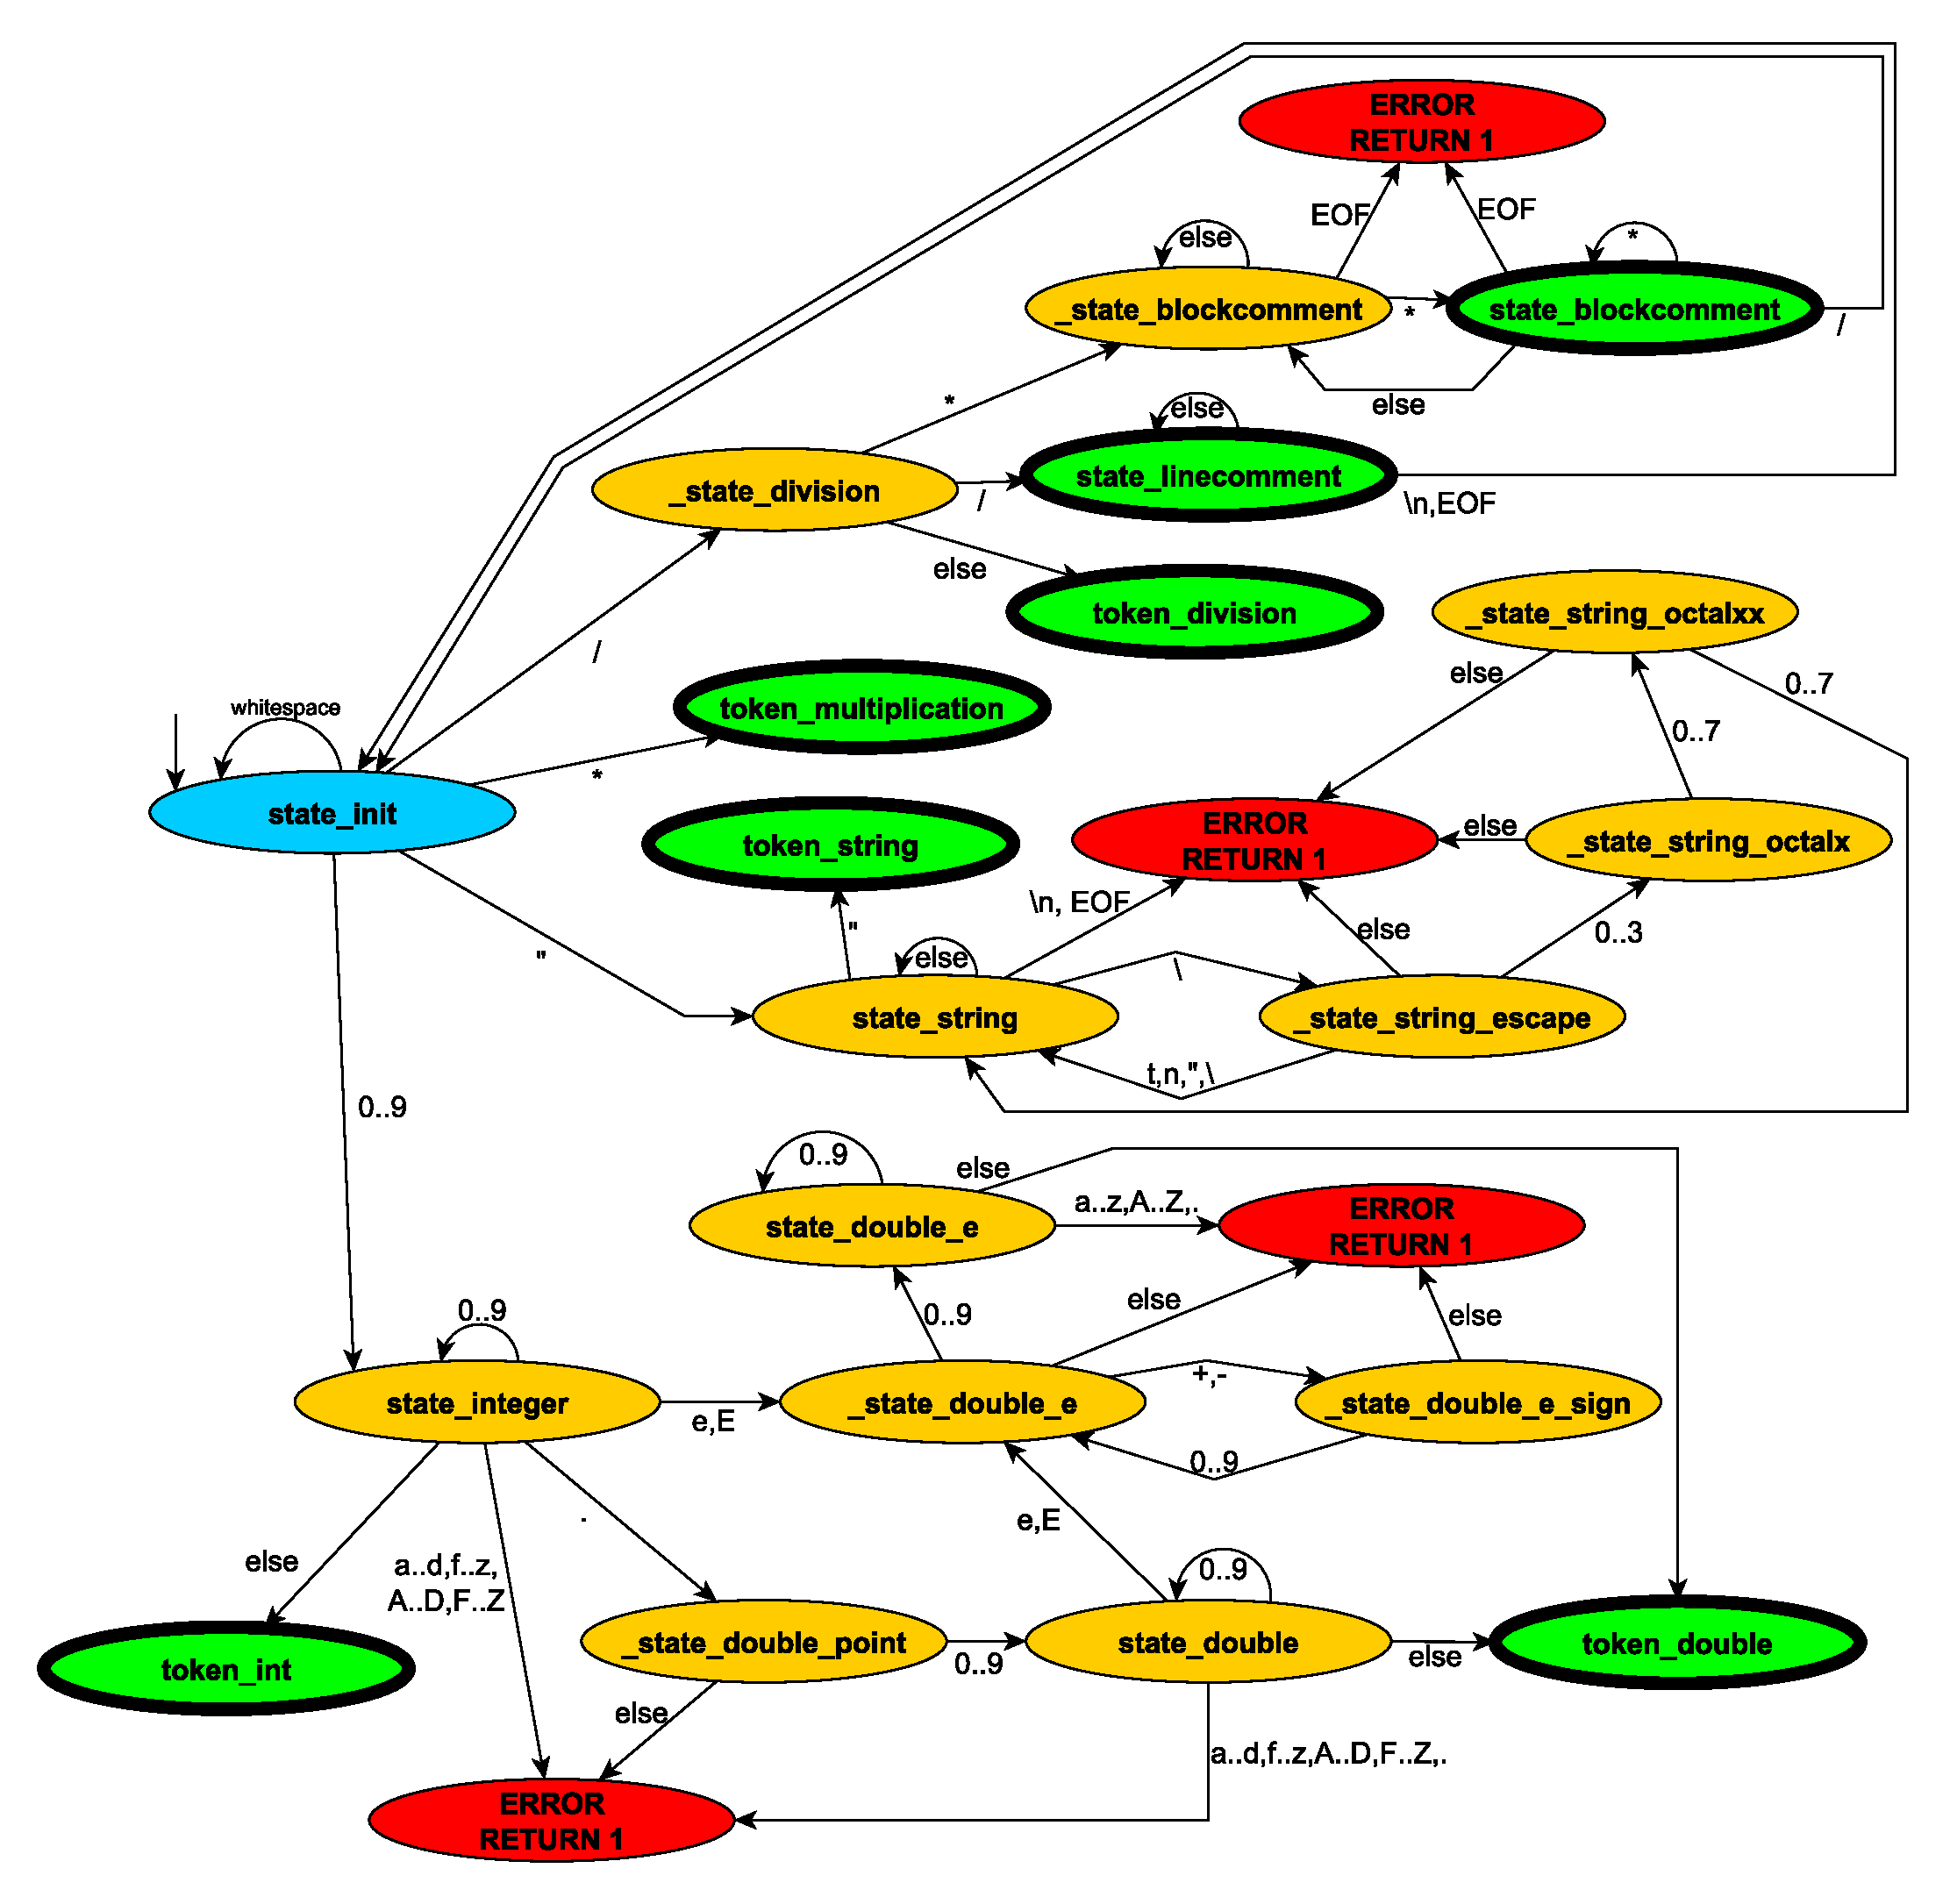
\includegraphics[scale=0.4]{docs/FSM_part1}
            \caption{Diagram konenečného automatu, část 1.}
        \end{figure}
        \begin{figure}[t]
		    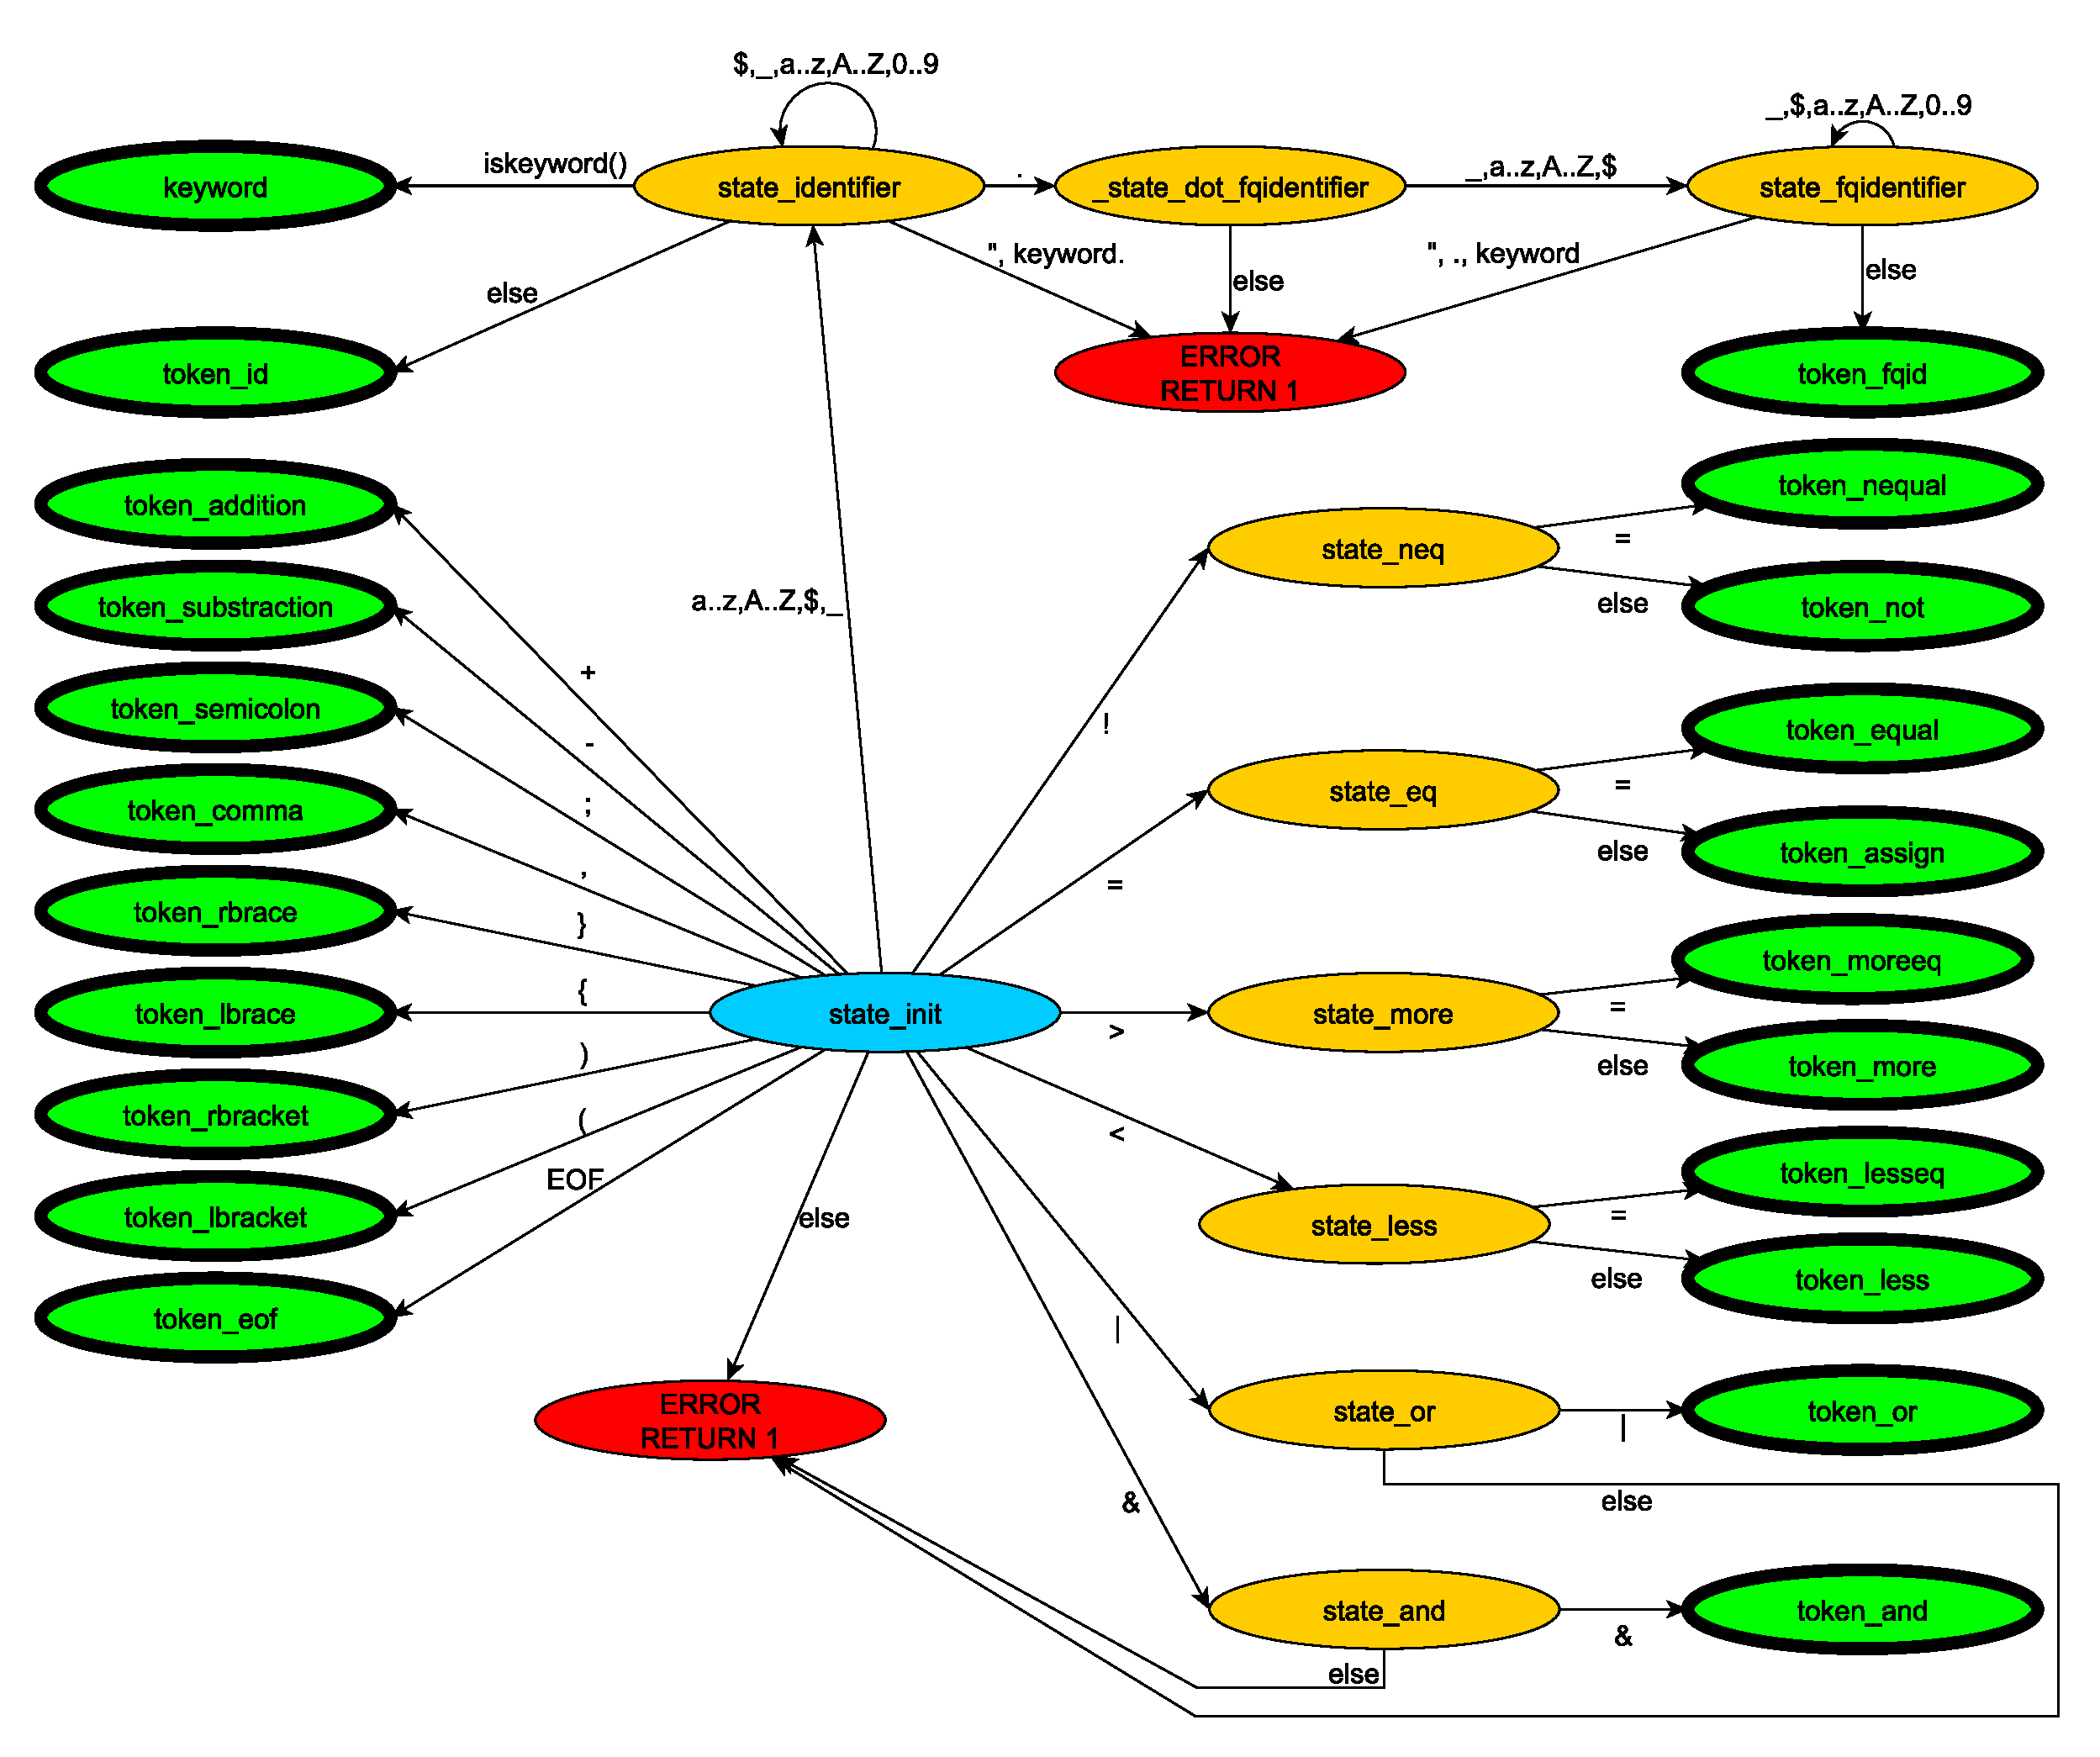
\includegraphics[scale=0.4]{docs/FSM_part2}
            \caption{Diagram konenečného automatu, část 2.}
        \end{figure}
	\end{center}
\end{document}
